\begin{titlepage}\centering
\vspace*{\fill}

\chapter{Exact compliance-based optimization with finitely many loading scenarios}\thispagestyle{EmptyHeader}
\label{chp:3}

\begin{tcolorbox}
This work is accepted for publication in the Journal of Structural and Multidisciplinary Optimization. The accepted manuscript can be found on arXiv (https://arxiv.org/abs/2103.04594). The paper is titled: "Robust and stochastic compliance-based topology optimization with finitely many loading scenarios"  \citep{tarek2021robust}
\end{tcolorbox}

\vspace*{\fill}
\end{titlepage}

\newpage

\section{Introduction}

Handling load uncertainty naively in topology optimization can prohibitively increase the computational cost of topology optimization. In this chapter, efficient methods to handle load uncertainty will be reviewed and novel ones will be proposed for compliance-based topology optimization.

\section{Literature review}

  \subsection{Mean compliance minimization}

    A number of works in literature tackled the problem of load uncertainty in compliance minimization problems. A general scheme for mean compliance minimization subject to uncertain load components with arbitrary covariance was proposed by \cite{Guest2008}. Guest et al. also considered uncertain load locations by treating the loaded nodes' locations as random and hence the stiffness matrix. Guest et al. then derived an approximately equivalent load distribution that would result in the same mean compliance while deterministically using the mean stiffness matrix. Mean compliance minimization subject to uncertainty of concentrated load magnitude and direction was studied by \cite{Dunning2011}. Dunning et al. derived efficient formulations for the mean compliance subject to such uncertainties, where the number of linear systems to be solved scales linearly with the number of independent random variables. This assumes that the distribution of the forces' magnitudes and rotations are known and independent. A similar formulation was then derived by \cite{Zhao2014} which requires fewer linear system solves per independent random variable. Zhao et al. also demonstrated how the same approach can handle distributed load uncertainty, modeled as a stochastic field, using Karhunen-Loeve (K-L) expansion. The main limitation of the K-L expansion method in practice is having to define and commit to a covariance kernel function. Additionally, the more local the covariance is, the higher the number of terms required in the K-L expansion to accurately describe the random field. The number of linear system solves required to compute the mean compliance scales with the number of terms in the K-L expansion.

    \cite{Zhang2017a} proposed an efficient way to compute the mean compliance for finitely many load scenarios with no assumptions about the nature of randomness. This can be used in data-driven design where the loading scenarios are many, and for which data has been collected. Alternatively, loading scenarios may be sampled from the distributions assumed if sufficiently low dimensional. Zhang et al. developed a randomized algorithm inspired by Hutchinson's trace estimator \cite{Hutchinson1990} to minimize the mean compliance: $\frac{1}{N} \sum_i^N \bm{f}^T_i \bm{K}^{-1} \bm{f}_i$, leading to significant computational savings compared to the naive approach. The algorithm can be trivially modified to handle weighted mean compliance which can be used in cases where the number of random variables are many following the approach by \cite{Zhao2014} or when the number of terms of the K-L expansion is high. The main limitation of this approach is that it can only be used to minimize the mean compliance which is not risk-averse since the compliance can be very high for some probable load scenarios. Finally, \cite{Liu2018a} solved the mean compliance minimization problem under a volume constraint subject to load uncertainty modeled using the fuzzy set theoretic cloud model for describing uncertainty.

  \subsection{Risk-averse compliance minimization}

    Beside mean compliance minimization, some authors also studied risk-averse compliance minimization by considering the weighted sum of the mean and variance, the weighted sum of the mean and standard deviation, as well as other risk measures. \cite{Dunning2013} derived an efficient formulation for the variance of the compliance subject to uncertainty in the load magnitude. This was used to minimize a weighted sum of the mean and variance of the compliance. The main limitation of this approach is that it cannot handle random load directions and that the distributions for the load magnitudes are assumed to be known and independent. \cite{Zhao2014b} minimized the weighted sum of the mean and standard deviation of the compliance by deriving an efficient formulation for the calculation of the mean and standard deviation of the compliance and their gradients under uncertain loading modeled as a random field. Zhao et al. used K-L expansion to quantify and describe the randomness using a few random variables, and used Monte Carlo simulation to calculate the fourth moment of those random variables which is required for the efficient computation of the standard deviation of the compliance.

    \cite{Chen2010} used the level-set method to minimize the weighted sum of the mean compliance and its variance subject to uncertainty in the load and material properties. Chen et al. assumed the load and material properties to be random fields and used K-L expansion to reduce their dimensionality. The authors then used Gaussian quadrature sampling to generate a representative set of scenarios to formulate the mean and variance of the compliance. \cite{Martinez-Frutos2016} used a similar uncertainty quantification approach to develop a multi-GPU density-based topology optimization framework for the large-scale minimization of the weighted sum of the mean compliance and its variance subject to load uncertainty only. However, Martinez-Frutos et al. used sparse grid sampling instead of Gaussian quadrature. Similarly, \cite{Cuellar2018} used K-L expansion for uncertainty quantification and Gaussian quadrature for sampling, and combined them with the non-intrusive polynomial chaos expansion (PCE) method to provide more accurate estimators for the mean and standard deviation of the compliance and their gradients. \cite{Martinez-Frutos2018} also used K-L expansion and the non-intrusive PCE with sparse grid sampling for the quantification and propagation of the uncertainty in the load and material properties. However, Martinez-Frutos et al. minimized a different compliance risk measure called the \textit{excess probability}, which is the probability that the compliance exceeds a certain threshold value. Note that in all the works above which use K-L expansion and sampling-based uncertainty propagation, the number of linear system solves can be made independent from the number of sampling points given the linearity assumption of the displacement as a function of the load exploited by \cite{Zhao2014b} in their derivation, even though in some of the works this property was not exploited. The number of linear system solves can therefore be assumed to be equal to the number of terms in the K-L expansion only, not the sampling points. 

    Also in risk-averse topology optimization, \cite{Garcia-Lopez2013} used multi-objective evolutionary optimization to optimize the mean and variance of the compliance and obtain the Pareto front of the two objectives. Garcia-Lopez et al. used a sampling method for uncertainty propagation inspired from Taguchi's method for the design of experiments. In this case, the number of linear system solves is equal to the number of sampling points. That beside the use of an evolutionary algorithm which requires many evaluations of the mean and variance of the compliance make the computational cost of this approach extremely high even for medium-sized problems. Finally, \cite{Kriegesmann2019} used FOSM instead of sampling to efficiently propagate the uncertainty estimating the mean and standard deviation of the compliance and their gradients from the means and standard deviations of the loads. A weighted sum of the mean and standard deviation of the compliance was then minimized. This approach assumes that the compliance is a linear function of the random load centered at the MPP load, an assumption which leads to a prediction error in the mean and standard deviation of the compliance. 

  \subsection{Probabilistic constraints and reliability-based topology optimization}

    \cite{Keshavarzzadeh2017} solved the problem of volume minimization subject to a probabilistic compliance constraint. In one case, the authors constrained the mean compliance plus a multiple of its standard deviation which is equivalent to a reliability constraint assuming the compliance is normally distributed. In another, a reliability constraint was used such that the probability that the compliance exceeds a threshold value is constrained. Keshavarzzadeh et al. used the non-intrusive PCE and regularized Heaviside function to approximate the compliance reliability constraint and its gradient. PCE was also used to estimate the mean and standard deviation of the compliance and their gradients.

    Beside sampling-based uncertainty propagation, RBDO offers a number of techniques for efficient, approximate uncertainty propagation which can be used for handling probabilistic constraints involving compliance or otherwise. \cite{Kharmanda2002,Kharmanda2004} proposed the use of RBDO for topology optimization, also known as reliability-based topology optimization (RBTO), to handle probabilistic constraints due to random loads, geometry and material properties. \cite{Jung2004} used FORM's PMA with SIMP topology optimization method to solve a volume minimization problem with a reliability constraint for geometrically nonlinear structures. The works by Kharmanda et al. and Jung et al. inspired other works such as \cite{Kim2006} who used FORM's RIA and PMA with SIMP to solve volume minimization problems with reliability constraints on the displacement and natural frequency of the structure under loading, material and geometry uncertainties. Another group, \cite{Kim2007,Kim2008}, later used RIA and PMA together with evolutionary structural optimization (ESO) \citep{YM1992,XY1998,Huang2010a} to solve volume minimization problems with a reliability constraint subject to a random load and Young's modulus. \cite{Ouyang2008} used FORM's RIA with the level-set method to solve a compliance minimization problem with a reliability constraint subject to uncertainty in the load and geometry of the ground mesh. 

    \cite{Silva2010} proposed the use of an efficiently obtainable approximate MPP to avoid the need for solving the reliability or inverse reliability problems in every design iteration of RIA or PMA, respectively. Silva et al. and later \cite{Nguyen2011} also considered system reliability-based topology optimization where an aggregated system failure probability is considered instead of component failure probabilities and component limit state functions. \cite{Zhao2016} presented a comparison of a number of RBTO approaches to solve a few topology optimization problems including one with a compliance reliability constraint under stochastic load and Young's modulus. \cite{Jalalpour2016} developed a bi-directional ESO (BESO) \citep{YM1992,XY1998,Huang2010a} algorithm for handling reliability constraints with displacement limit state functions and a finite number of probable loading scenarios in linearly elastic structures. Finally, \cite{Yin2018} proposed an alternative RBTO approach using fuzzy set theory to describe the uncertainty.

  \subsection{Maximum compliance constraint}

    Beside the stochastic and risk-averse topology optimization presented above, a number of works also studied maximum compliance minimization and maximum compliance constrained problems under uncertain loading conditions, where the former can be formulated using the latter as shown earlier. In these papers, no probability distribution is assumed for the uncertain load and therefore they fall under the category of RO. Most of the work on handling non-probabilistic uncertainty in loads assumed that the loads lie in continuous sets. \cite{Brittain2012} for example assumed that the load vector has a fixed norm but arbitrary direction. Brittain et al. used a bi-level min-max optimization approach minimizing the objective with respect to the topology variables in the upper level problem, and maximizing with respect to the load in the lower level problem. However, an efficient algorithm was derived for the lower level maximization problem based on the KKT optimality conditions for the objective and the load's fixed-norm constraint. \cite{Holmberg2015} proposed a nonlinear semidefinite formulation to solve the maximum compliance minimization problem under non-probabilistic load uncertainty, assuming the uncertain load lies in a hyper-ellipsoid uncertainty set:
    \begin{align}
      & \bm{f} = \bm{f}_0 + \bm{Q} \bm{r} \\
      & ||\bm{r}|| \leq 1
    \end{align}
    where $\bm{f}_0$ is the fixed component of the load vector and the columns of $\bm{Q}$ are the axes of the uncertainty hyper-ellipsoid. The same authors, \cite{Thore2017}, later generalized their approach from \cite{Holmberg2015} to handle maximum compliance and maximum stress constraints under the same assumption on the load vector. Similarly, \cite{Liu2018} proposed a bi-level formulation for handling multiple independent loads, each of which lies in a hyper-ellipsoidal uncertainty set. Liu et al. developed an efficient lower level algorithm by solving the Wolfe dual problem. The Wolfe dual problem of the lower level problem is a maximum generalized eigenvalue minimization problem which was solved using an iterative procedure. The multi-ellipsoidal uncertainty set generalizes the interval as well as the spherical uncertainty sets.

    A number of papers were also published on non-probabilistic reliability-based topology optimization (NRBTO) where new reliability indexes and performance measures are defined for various types of continuous uncertainty sets. While some of these works did not solve problems with maximum compliance constraints, but the same techniques can be applied to handle maximum compliance constraints. \cite{Luo2009} proposed a reliability index and performance measure for handling non-probabilistic uncertainty where the uncertain variables lie in a multi-ellipsoid model. Another reliability index for ellipsoidal uncertainty was then proposed by \cite{Wang2018a}. \cite{Wang2017,Wang2019a} proposed another reliability index for handling interval uncertainty sets using interval arithmetic. \cite{Zheng2018a} proposed a reliability index and performance function for uncertain variables in multidimensional parallelepiped convex sets. Another reliability index for mixed interval and ellipsoidal uncertainty was also developed by \cite{Wang2019b}.

    The rest of this chapter is organized as follows. The proposed approaches for handling load uncertainty in continuum compliance problems in the form of a large, finite number of loading scenarios are detailed in sections \ref{sec:proposed_mean}, \ref{sec:proposed_risk} and \ref{sec:proposed_max}. The experiments used and the implementations are then described in section \ref{sec:exp_impl}. Finally, the results are presented and discussed in section \ref{sec:results} before concluding in section \ref{sec:conclusion}.

\section{Compliance sample mean and its gradient} \label{sec:proposed_mean}

  \subsection{Naive approach}

    The compliance sample mean for a finite number $L$ of loading scenarios is $\mu_C = \frac{1}{L} \sum_{i=1}^L \bm{f}_i^T \bm{K}^{-1} \bm{f}_i$ where $\bm{f}_i$ is the $i^{th}$ load scenario, $\bm{K}$ is the stiffness matrix of the design and $\bm{F}$ is the matrix whose columns are the individual loading scenarios $\bm{f}_i$. The direct naive approach is to solve for $\bm{K}^{-1} \bm{f}_i$ for all $i$ and calculate the mean compliance using the above formula. This method is not efficient since it requires $L$ linear system solves plus some additional work to compute the mean with a time complexity of $O(L \times n_{dofs})$, where $n_{dofs}$ is the number of degrees of freedom in the design. When $\bm{F}$ is sparse with only a few $n_{loaded}$ degrees of freedom that are loaded, the complexity of the remaining work to compute the mean compliance $\frac{1}{L} \sum_{i=1}^L \bm{f}_i^T \bm{u}_i$ becomes $O(L \times n_{loaded})$. Even though the factorization of $\bm{K}^{-1}$ can be reused to solve for the $L$ linear systems, if $L$ is close to $n_{dofs}$, the complexity of solving for so many linear systems will be similar to that of the factorization, thus significantly adding to the running time. When using an iterative algorithm to solve for $\bm{K}^{-1}\bm{f}_i$, a good, but expensively formed, preconditioner such as the algebraic multi-grid preconditioner can be similarly reused. In general, significantly reducing the number of linear systems to solve is advantageous in practice even if, as theory may show, the running time is dominated by the initial linear system solve.

    Let the Jacobian of $\bm{\rho}(\bm{x})$ be $\nabla_{\bm{x}} \bm{\rho}(\bm{x})$. Let $\bm{u}_i$ be the displacement response due to load $\bm{f}_i$ and $C_i$ be the compliance $\bm{f}_i^T \bm{u}_i$. The stiffness matrix $\bm{K}$ is typically defined as: $\bm{K} = \sum_e \rho_e \bm{K}_e$. The partial derivative of the compliance $C_i$ with respect to $\rho_e$ is given by $\frac{\partial C_i}{\partial \rho_e} = -\bm{u}_i^T \bm{K}_e \bm{u}_i$. The gradient of $C_i$ with respect to the decision vector $\bm{x}$ is therefore given by: $\nabla_{\bm{x}} C_i(\bm{x}) = \nabla_{\bm{x}} \bm{\rho}(\bm{x})^T \nabla_{\bm{\rho}} C_i(\bm{\rho}(\bm{x}))$ where $\nabla_{\bm{\rho}} C_i(\bm{\rho}(\bm{x}))$ is the gradient of $C_i$ with respect to $\bm{\rho}$ at $\bm{\rho}(\bm{x})$. The gradient of the mean compliance $\mu_C$ is therefore given by $\nabla_{\bm{x}} \mu_C(\bm{x}) = \frac{1}{L} \sum_{i=1}^L \nabla_{\bm{x}} \bm{\rho}(\bm{x})^T \nabla_{\bm{\rho}} C_i(\bm{\rho}(\bm{x}))$. The additional complexity of computing the mean compliance and its gradient with respect to $\bm{\rho}$ is $O(n_E \times L)$. Note that the Jacobian of $\bm{\rho}(\bm{x})$ does not need to be formed explicitly to compute the gradient above, so long as there is a way to pre-multiply the Jacobian's transpose by a vector. The problem with the naive approach is it requires many linear system solves and so doesn't scale well to many loading scenarios.

  \subsection{Singular value decomposition}

    Less naively, one can first attempt to find the singular value decomposition (SVD) of $\bm{F}$. Let the compact SVD of the matrix $\bm{F}$ be $\bm{F} = \bm{U} \bm{S} \bm{V}^T$, where the number of non-zero singular values is $n_s$, $\bm{S}$ is the diagonal matrix of singular values, $\bm{U}$ is a $n_{dofs} \times n_s$ matrix with orthonormal columns, and $\bm{V}$ is $L \times n_s$ matrix with orthonormal columns. Given the SVD, the mean compliance can be written as: $\mu_C = \frac{1}{L} \sum_{i=1}^L \bm{f}_i^T \bm{K}^{-1} \bm{f}_i = \frac{1}{L} tr(\bm{F}^T \bm{K}^{-1} \bm{F})$. This can be further simplified:
    \begin{align}
     \frac{1}{L} tr(\bm{F}^T \bm{K}^{-1} \bm{F}) & = \frac{1}{L} tr(\bm{V} \bm{S} \bm{U}^T \bm{K}^{-1} \bm{U} \bm{S} \bm{V}^T) \\
     & = \frac{1}{L} tr(\bm{S} \bm{U}^T \bm{K}^{-1} \bm{U} \bm{S}) \\
     & = \frac{1}{L} \sum_{i=1}^{n_s} \bm{S}[i,i]^2 \times \bm{U}[:,i]^T \bm{K}^{-1} \bm{U}[:,i]
    \end{align}
    This method requires only $n_s$ linear system solves and an SVD. $n_s$ will be small if the loads in $\bm{F}$ are highly correlated or if only a few degrees of freedom are loaded, i.e. the loads are sparse. Let $n_{loaded}$ be the few loaded degrees of freedom. It is possible to prove in this case that the number of singular values $n_s \leq n_{loaded}$. The computational time complexity of computing the SVD of $\bm{F}$ in the dense case is $O(min(L, n_{dofs})^2 max(L, n_{dofs}))$, while in the sparse case it is only $O(n_{loaded}^2 L)$. If $n_{loaded}$ is a small constant, finding the SVD will be very efficient. Additionally, when only $n_{loaded}$ degrees of freedom are loaded in $\bm{F}$, only the same degrees of freedom will be non-zero in $\bm{U}$, therefore $\bm{U}$ will also be sparse. Other than the complexity of SVD, the additional work to compute the mean compliance has a computational time complexity of $O(n_s \times n_{dofs})$ when $\bm{F}$ (and $\bm{U}$) are dense, and $O(n_s \times n_{loaded})$ when $\bm{F}$ (and $\bm{U}$) are sparse.

    Given the efficient formula for the mean compliance and using the derivative rule of the inverse quadratic from appendix section \ref{app1}, the partial $\frac{\partial \mu_C}{\partial \rho_e}$ is given by: \\ $-\frac{1}{L} \sum_{i=1}^{n_s} \bm{S}[i,i]^2 (\bm{K}^{-1}\bm{U})[:,i]^T \bm{K}_e (\bm{K}^{-1}\bm{U})[:,i]$. The time complexity of computing this assuming we already computed $\bm{K}^{-1} \bm{U}$ is $O(n_s \times n_E)$. 

  \begin{table*}[h!]
   \centering
   \caption{Summary of the computational cost of the algorithms discussed to calculate the mean compliance and its gradient. \#Lin is the number of linear system solves required.}
   \begin{tabular}{| m{1.7cm} | m{0.7cm} | m{1.0cm} | m{4cm} | m{4cm}|} 
    \hline
    \multirow{2}{3em}{Method} & \multirow{2}{2em}{\#Lin} & \multirow{2}{2em}{SVD?} & \multicolumn{2}{c|}{Time complexity of additional work} \\\cline{4-5}
    & & & Dense & Sparse \\
    \hline
    \hline
    Exact-Naive & \(L\) & \xmark & \(O(L \times (n_{dofs} + n_E))\) & \(O(L \times (n_{loaded} + n_E))\) \\
    \hline
    Exact-SVD & \(n_s\) & \cmark & \(O(n_s \times (n_{dofs} + n_E))\) & \(O(n_s \times (n_{loaded} + n_E))\) \\
    \hline
   \end{tabular}
   \label{tab:perf_mean}
  \end{table*}

\section{Scalar-valued function of load compliances and its gradient} \label{sec:proposed_risk}

  In this section, the above approach for computing the sample mean compliance will be generalized to handle the sample variance and standard deviations. The sample variance of the compliance $C$ is given by $\sigma_C^2 = \frac{1}{L-1} \sum_{i=1}^L (C_i - \mu_C)^2$. The sample standard deviation $\sigma_C$ is the square root of the variance. Let $\bm{C}$ be the vector of compliances $C_i$, one for each load scenario. In vector form, $\sigma_C^2 = \frac{1}{L-1} (\bm{C} - \mu_C \bm{1})^T (\bm{C} - \mu_C \bm{1})$. $\bm{C} = diag(\bm{A})$ is the diagonal of the matrix $\bm{A} = \bm{F}^T \bm{K}^{-1} \bm{F}$.

  \subsection{Naive approach}

    If one can compute the vector of load compliances $\bm{C}$, computing the variance and standard deviation is trivial. This approach requires $L$ linear system solves which can be computationally prohibitive if $L$ is large. Other than the linear system solves, the remaining work of computing $C_i = \bm{f}_i^T \bm{u}_i$ for all $i$ has a complexity of $O(L \times n_{dofs})$ when $\bm{F}$ is dense and $O(L \times n_{loaded})$ when $\bm{F}$ is sparse with only $n_{loaded}$ loaded degrees of freedom. In order to compute the vector $\bm{C}$ exactly, one needs to compute $\bm{u}_i = \bm{K}^{-1} \bm{f}_i$ for all $i$. These can further be used to compute the gradients of the load compliances $C_i$ which can be combined to form the Jacobian $\nabla_{\bm{\rho}} \bm{C}$. Assuming $\bm{u}_i$ is cached for all $i$, the time complexity of computing the Jacobian using $\frac{\partial C_i}{\partial \rho_e} = -\bm{u}_i^T \bm{K}_e \bm{u}_i$ is $O(n_E \times L)$.

    However, when interested in the gradient of a scalar-valued function $f$ of $\bm{C}$, there is no need to form the full Jacobian $\nabla_{\bm{x}} \bm{C}(\bm{x})$. It suffices to define an operator to pre-multiply an arbitrary vector $\bm{w}$ by $\nabla_{\bm{x}} \bm{C}(\bm{x})^T$. Using the chain rule, the gradient of $f$ with respect to $\bm{x}$ is given by $\nabla_{\bm{x}} f(\bm{C}(\bm{x})) = \nabla_{\bm{x}} \bm{C}(\bm{x})^T \nabla_{\bm{C}} f(\bm{C}(\bm{x}))$. This operator is equivalent to attempting to find the gradient of the weighted sum of $\bm{C}$, $\bm{w}^T \bm{C}$, where $\bm{w}$ is the constant vector of weights. In the case of a general scalar-valued function $f$, $\bm{w}$ would be $\nabla_{\bm{C}} f(\bm{C}(\bm{x}))$ and is treated as a constant. In the case of the variance, $f(\bm{C}) = \sigma_C^2 = \frac{1}{L-1} (\bm{C} - \mu_C \bm{1})^T (\bm{C} - \mu_C \bm{1})$, therefore $\bm{w} = \nabla_{\bm{C}} f(\bm{C}(\bm{x})) = \frac{2}{L-1} (\bm{C} - \mu_C \bm{1})$. And in the case of the standard deviation $\sigma_C$, $\bm{w} = \frac{1}{(L-1)\sigma_C} (\bm{C} - \mu_C \bm{1})$. This means that computing $\bm{C}$ is required to form $\bm{w}$.

    By caching $\bm{u}_i = \bm{K}^{-1}\bm{f}_i$ for all $i$ when computing $\bm{C}$, one can find the $e^{th}$ element of $\nabla_{\bm{x}} \bm{C}(\bm{x})^T \bm{w}$ using $\sum_{i=1}^L -w_i \bm{u}_i^T \bm{K}_e \bm{u}_i$, where $w_i$ is $i^{th}$ element of $\bm{w}$. Computing $\bm{u}_i^T \bm{K}_e \bm{u}_i$ requires constant time complexity, therefore the additional time complexity of computing $\nabla_{\bm{x}} \bm{C}(\bm{x})^T \bm{w}$ after computing $\bm{C}$ with the direct method is $O(L \times n_E)$. In this case, this is the same complexity as forming the Jacobian first and then multiplying, but in the next algorithms, it will be different.

  \subsection{Singular value decomposition}

    Much like in the mean compliance calculation, the SVD of $\bm{F}$ can be computed to find $C_i$ for all $i$ more efficiently from $\bm{K}^{-1} \bm{U} \bm{S}$. The number of linear system solves required to compute $\bm{K}^{-1} \bm{U} \bm{S}$ is $n_s$, the number of singular values of $\bm{F}$. The computational cost of computing $C_i = \bm{f}_i^T \bm{u}_i = \bm{f}_i^T (\bm{K}^{-1} \bm{U} \bm{S}) V^T[:,i]$ for all $i$ using $\bm{K}^{-1} \bm{U} \bm{S}$ and $\bm{V}$ is $O(L \times n_s \times n_{dofs})$ when $\bm{F}$ is dense and $O(L \times n_s \times n_{loaded})$ when $\bm{F}$ is sparse with only $n_{loaded}$ degrees of freedom loaded. The Jacobian $\nabla_{\bm{\rho}} \bm{C}$ can be built by first computing $\bm{K}^{-1} \bm{F}$ from the cached $\bm{K}^{-1} \bm{U} \bm{S}$ then using it much like in the exact method without SVD. This has a time complexity of $O((n_s \times n_{dofs} + n_E) \times L)$.

    However, when interested in $\nabla_{\bm{\rho}} \bm{C}^T \bm{w}$ instead, a more efficient approach can be used. Let $\bm{D}_{\bm{w}}$ be the diagonal matrix with the vector $\bm{w}$ on the diagonal.
    \begin{align}
     \nabla_{\bm{\rho}} \bm{C}^T \bm{w} & = \nabla_{\bm{\rho}} (\bm{C}^T \bm{w}) = \nabla_{\bm{\rho}} tr(\bm{D}_{\bm{w}} \bm{F}^T \bm{K}^{-1} \bm{F}) \\
     & = \nabla_{\bm{\rho}} tr(\bm{V}^T \bm{D}_{\bm{w}} \bm{V} \bm{S} \bm{U}^T \bm{K}^{-1} \bm{U} \bm{S})
    \end{align}
    Let $\bm{X} = \bm{V}^T \bm{D}_{\bm{w}} \bm{V}$ and $\bm{Q} = \bm{K}^{-1} \bm{U} \bm{S}$. The partial derivative of the above with respect to $\rho_e$ is:
    \begin{align}
     & \frac{\partial}{\partial \rho_e} tr(\bm{X} \bm{Q}^T \bm{S} \bm{U}^T \bm{K}^{-1} \bm{U} \bm{S}) = -tr(\bm{X} \bm{Q}^T \bm{K}_e \bm{Q})
    \end{align}

    Note that one can cache $\bm{Q} = \bm{K}^{-1} \bm{U} \bm{S}$ when finding the function value above to be reused in the sensitivity analysis. Let $\bm{Y}_e = \bm{Q}^T \bm{K}_e \bm{Q}$. The trace above is therefore $tr(\bm{X} \bm{Y}_e) = tr(\bm{X}^T \bm{Y}_e) = \sum_{i=1}^{n_s} \sum_{j=1}^{n_s} \bm{X}[i,j] \times \bm{Y}_e[i,j]$. Computing $\bm{Y}_e[i,j]$ from the pre-computed $\bm{Q}$ requires a constant time complexity for each element $e$, and computing $\bm{X}$ has a time complexity of $O(L \times n_s^2)$. The additional time complexity of computing $\nabla_{\bm{\rho}} \bm{C}^T \bm{w}$ using this method is therefore $O((n_E + L) \times n_s^2)$. So if $n_s \ll L$, significant computational savings can be made compared to directly computing the Jacobian then doing the matrix-vector multiplication $\nabla_{\bm{\rho}} \bm{C}^T \bm{w}$ which has a complexity of $O((n_s \times n_{dofs} + n_E) \times L)$.

    \begin{table*}[h!]
      \centering
      \caption{Summary of the computational cost of the algorithms discussed to calculate the load compliances $\bm{C}$ as well as $\nabla_{\bm{\rho}} \bm{C}^T \bm{w}$ for any vector $\bm{w}$. \#Lin is the number of linear system solves required. This can be used to compute the variance, standard deviation as well as other scalar-valued functions of $\bm{C}$. If the full Jacobian is required, the naive method requires the same computational cost as that of computing $\nabla_{\bm{\rho}} \bm{C}^T \bm{w}$, and the SVD-based method has a time complexity of $O((n_s \times n_{dofs} + n_E) \times L)$ for the additional work other than the linear system solves and SVD.}
      \begin{tabular}{|m{1.7cm} | m{0.7cm} | m{0.8cm} | m{5.0cm} | m{5.0cm} |} 
       \hline
       \multirow{2}{3em}{Method} & \multirow{2}{2em}{\#Lin} & \multirow{2}{2em}{SVD?} & \multicolumn{2}{c|}{Time complexity of additional work} \\\cline{4-5}
       & & & Dense & Sparse \\
       \hline
       \hline
       Exact-Naive & \(L\) & \xmark & \(O(L \times (n_{dofs} + n_E))\) & \(O(L \times (n_{loaded} + n_E))\) \\
       \hline
       Exact-SVD & \(n_s\) & \cmark & \(O(L \times n_s \times n_{dofs} + (n_E + L) \times n_s^2)\) & \(O(L \times n_s \times n_{loaded} + (n_E + L) \times n_s^2)\) \\
      \hline
     \end{tabular}
     \label{tab:perf_scalar}
    \end{table*}

\section{Maximum compliance constraint} \label{sec:proposed_max}

  The maximum compliance constraint can be efficiently handled using the augmented Lagrangian optimization algorithm \citep{Bertsekas1996}. Assume the following maximum compliance constrained problem is to be solved for some objective $g(\bm{x})$ using the augmented Lagrangian algorithm:
  \begin{mini!}|l|[3]
    {\bm{x}}{g(\bm{x})}{}{}
    \addConstraint {\quad C_i = \bm{f}_i^T \bm{K}^{-1} \bm{f}_i \leq C_t}{\quad \forall i \in 1 \dots L}
    \addConstraint {0 \leq x_e \leq 1}{\quad \forall e \in 1 \dots n_E}
  \end{mini!}
  where $C_t$ is the maximum compliance allowed. In the augmented Lagrangian algorithm, the problem is transformed as follows:
  \begin{mini!}|l|[3]
    {\bm{x}}{L(\bm{x}; \bm{\lambda}, r)}{}{}
    \addConstraint {0 \leq x_e \leq 1}{\quad \forall e \in 1 \dots n_E}
  \end{mini!}
  \begin{align}
    L(\bm{x}; \bm{\lambda}, r) = g(\bm{x}) + \sum_{i=1}^{L} \biggl( \lambda_i (C_i - C_t) + r \max(C_i - C_t, 0)^2 \biggr)
  \end{align}
  where $\bm{\lambda}$ is the vector of Lagrangian multipliers $\lambda_i$, one for each compliance constraint, and $r$ is the constant coefficient of the quadratic penalty. Solving the above problem using a first-order box constrained algorithm requires the gradient of $L(\bm{x})$. Writing $L(\bm{x})$ in vector form:
  \begin{align}
    L(\bm{x}) = g(\bm{x}) + \bm{\lambda}^T (\bm{C} - C_t \bm{1}) + r \bm{M}' \bm{M}
  \end{align}
  where $\bm{M}$ is the vector whose $i^{th}$ element is $max(C_i - C_t, 0)$. The gradient of $L(\bm{x})$ is given by:
  \begin{align}
    \nabla_{\bm{x}} L(\bm{x}) & = \nabla_{\bm{x}} g + \nabla_{\bm{x}} \bm{\rho}^T (\nabla_{\bm{\rho}} (\bm{\lambda}^T (\bm{C} - C_t \bm{1}) + r \bm{M}' \bm{M}) \\
    & = \nabla_{\bm{x}} g + \nabla_{\bm{x}} \bm{\rho}^T \nabla_{\bm{\rho}} \bm{C}^T (\bm{\lambda} + 2 \bm{M})
  \end{align}
  As shown in the previous sections, calculating the product $\nabla_{\bm{\rho}} \bm{C}^T (\bm{\lambda} + 2 \bm{M})$ can be done efficiently by finding the gradient $\nabla_{\bm{\rho}} (\bm{C}^T \bm{w})$ using $\bm{w} = (\bm{\lambda} + 2 \bm{M})$. Therefore, the results from Table \ref{tab:perf_scalar} apply.

\section{Setup and Implementation} \label{sec:exp_impl}

  In this section, the most important implementation details and algorithm settings used in the experiments are presented.

  \subsection{Test problems}

    \subsubsection{2D cantilever beam}

      \begin{figure}
  \centering
  \resizebox{\textwidth}{!}{
    \begin{tikzpicture}
        \draw[fill,color=gray!70] (0,-0.1) rectangle (-0.3,2.1);
        \node [align=center, body,line width=1.2pt,minimum height=2cm,minimum width=8cm,anchor=south west] (body1) at (0,0) {};
        \draw (body1.south east) -- ++(1.6,0) coordinate (D1) -- +(5pt,0);
        \draw (body1.north east) -- ++(1.6,0) coordinate (D2) -- +(5pt,0);
        \draw [dimen] (D1) -- (D2) node {40mm};

        \draw (body1.north west) -- ++(0,2) coordinate (D1) -- +(0,5pt);
        \draw (body1.north east) -- ++(0,2) coordinate (D2) -- +(0,5pt);
        \draw [dimen] (D1) -- (D2) node {160mm};

        \draw[->,line width=1pt] (8,1) -- (9,1) -- (9,0.2);
        \node (arrowhead) at (8.7,0.25) {$\bm{F}_1$};

        \draw (body1.north west) -- ++(0,1.5) coordinate (D1) -- +(0,5pt);
        \draw (4,2) -- ++(0,1.5) coordinate (D2) -- +(0,5pt);
        \draw [dimen] (D1) -- (D2) node {80mm};

        \draw[->,line width=1pt] (3.4,2.6) -- (4,2);
        \node (arrowhead) at (3.2,2.8) {$\bm{F}_2$};

        \draw (body1.south west) -- ++(0,-1.5) coordinate (D1) -- +(0,5pt);
        \draw (6,0) -- ++(0,-1.5) coordinate (D2) -- +(0,5pt);
        \draw [dimen] (D1) -- (D2) node {120mm};

        \draw[->,line width=1pt] (6,0) -- (5.4,-0.6);
        \node (arrowhead) at (5.2,-0.8) {$\bm{F}_3$};

        \draw[->,line width=1pt] (0.3,2.3) -- (0.1,2);
        \draw[->,line width=1pt] (0.6,2.3) -- (0.8,2);
        \draw[->,line width=1pt] (1.2,2.3) -- (1.1,2);
        \draw[->,line width=1pt] (1.5,2.3) -- (1.8,2);
        \draw[->,line width=1pt] (2.2,2.3) -- (2.0,2);
        \draw[->,line width=1pt] (2.5,2.3) -- (2.8,2);
        \draw[->,line width=1pt] (3.1,2.3) -- (3.0,2);
        \draw[->,line width=1pt] (3.3,2.3) -- (3.5,2);
        \draw[->,line width=1pt] (4.5,2.3) -- (4.4,2);
        \draw[->,line width=1pt] (4.8,2.3) -- (4.9,2);
        \draw[->,line width=1pt] (5.3,2.3) -- (5.1,2);
        \draw[->,line width=1pt] (5.6,2.3) -- (5.9,2);
        \draw[->,line width=1pt] (6.2,2.3) -- (6.0,2);
        \draw[->,line width=1pt] (6.5,2.3) -- (6.9,2);
        \draw[->,line width=1pt] (7.2,2.3) -- (7.2,2);
        \draw[->,line width=1pt] (7.5,2.3) -- (7.7,2);
        \draw[->,line width=1pt] (8.1,2.3) -- (7.9,2);

        \draw[->,line width=1pt] (0.3,-0.3) -- (0.3,0);
        \draw[->,line width=1pt] (0.8,-0.3) -- (0.6,0);
        \draw[->,line width=1pt] (1.2,-0.3) -- (1.1,0);
        \draw[->,line width=1pt] (1.5,-0.3) -- (1.5,0);
        \draw[->,line width=1pt] (2.0,-0.3) -- (2.2,0);
        \draw[->,line width=1pt] (2.5,-0.3) -- (2.8,0);
        \draw[->,line width=1pt] (3.1,-0.3) -- (3.0,0);
        \draw[->,line width=1pt] (3.5,-0.3) -- (3.2,0);
        \draw[->,line width=1pt] (3.8,-0.3) -- (3.7,0);
        \draw[->,line width=1pt] (4.1,-0.3) -- (4.1,0);
        \draw[->,line width=1pt] (4.4,-0.3) -- (4.4,0);
        \draw[->,line width=1pt] (5.0,-0.3) -- (4.9,0);
        \draw[->,line width=1pt] (5.3,-0.3) -- (5.3,0);
        \draw[->,line width=1pt] (5.5,-0.3) -- (5.6,0);
        \draw[->,line width=1pt] (6.0,-0.3) -- (6.2,0);
        \draw[->,line width=1pt] (6.6,-0.3) -- (6.7,0);
        \draw[->,line width=1pt] (7.3,-0.3) -- (7.2,0);
        \draw[->,line width=1pt] (7.7,-0.3) -- (7.5,0);
        \draw[->,line width=1pt] (8.1,-0.3) -- (7.9,0);

        \draw[->,line width=1pt] (8.3,0.3) -- (8.0,0.1);
        \draw[->,line width=1pt] (8.3,0.5) -- (8.0,0.8);
        \draw[->,line width=1pt] (8.3,1.0) -- (8.0,1.2);
        \draw[->,line width=1pt] (8.3,1.5) -- (8.0,1.5);
        \draw[->,line width=1pt] (8.3,1.7) -- (8.0,1.9);
    \end{tikzpicture} \newline
  }
  \caption{Cantilever beam problem. $\bm{F}_2$ and $\bm{F}_3$ are at 45 degree angles.}
  \label{fig:CantBeam}
\end{figure}


      The 2D cantilever beam problem shown in Figure \ref{fig:CantBeam} was used to run the experiments. A ground mesh of plane stress quadrilateral elements was used, where each element is a square of side length $1 \text{ mm}$, and a sheet thickness of $1 \text{ mm}$. Linear iso-parametric interpolation functions were used for the field and geometric basis functions. A Young's modulus of 1 MPa and Poisson's ratio of 0.3 were used. Finally, a chequerboard density filter for unstructured meshes was used with a radius of 2 mm \citep{Huang2010a}. A 3D version of the problem above was also solved. Details of the 3D problem and the results are shown in appendix section \ref{app1}.

      Three variants of the cantilever beam problem were solved:
      \begin{enumerate}
        \item Minimization of the mean compliance $\mu_C$ subject to a volume constraint with a volume fraction of 0.4,
        \item Minimization of a weighted sum of the mean and standard deviation (mean-std) of the compliance $\mu_C + 2.0 \sigma_C$ subject to a volume constraint with a volume fraction of 0.4, and
        \item Volume minimization subject to a maximum compliance constraint with a compliance threshold of $70000 \text{ Nmm}$.
      \end{enumerate}
      A total of 1000 load scenarios were sampled from:
      \begin{align}
        \bm{f}_i = s_1 \bm{F}_1 + s_2 \bm{F}_2 + s_3 \bm{F}_3 + \frac{1}{7} \sum_{j=4}^{10} s_j \bm{F}_j
      \end{align}
      where $\bm{F}_1$, $\bm{F}_2$ and $\bm{F}_3$ are unit vectors with directions as shown in Figure \ref{fig:CantBeam}. $\bm{F}_2$ and $\bm{F}_3$ are at 45 degrees. $s_1$, $s_2$ and $s_3$ are identically and independently uniformly distributed random variables between -2 and 2. $\bm{F}_j$ for $j$ in $4 \dots 10$ are vectors with non-zeros at all the surface degrees of freedom without a Dirichlet boundary condition. The non-zero values are identically and independently normally distributed random variables with mean 0 and standard deviation 1. $s_j$ for $j$ in $4 \dots 10$ are also identically and independently normally distributed random variables with mean 0 and standard deviation 1. The same loading scenarios were used for the 3 test problems. Let $\bm{F}$ be the matrix whose columns are the sampled $\bm{f}_i$ vectors. The way the loading scenarios are defined, the rank of $\bm{F}$ can be at most 10 and was actually exactly 10 in our experiments. Given the low rank structure of $\bm{F}$, the SVD approaches should be expected to be significantly more efficient than their naive counterparts.

    \subsubsection{3D cantilever beam}

      A 3D version of the 2D cantilever beam test problem above was also solved using the methods proposed. A 60 mm x 20 mm x 20 mm 3D cantilever beam was used with hexahedral elements of cubic shape and side length of 1 mm. The loads $\bm{F}_1$, $\bm{F}_2$ and $\bm{F}_3$ were positioned at (60, 10, 10), (30, 20, 10) and (40, 0, 10) where the coordinates represent the length, height and depth respectively. The remaining loads and multipliers were sampled from the same distributions as the 2D problem. A density filter radius of 3 mm was also used for the 3D problem.

  \subsection{Settings}

    The value of $x_{min}$ used was $0.001$ for all problems and algorithms. Penalization was done prior to interpolation to calculate $\bm{\rho}$ from $\bm{x}$. A power penalty function and a regularized Heaviside projection were used. All of the problems were solved using 2 continuation SIMP routines. The first incremented the penalty value from $p = 1$ to $p = 6$ in increments of 0.5. Then the Heaviside projection parameter $\beta$ was incremented from $\beta = 0$ to $\beta = 20$ in increments of 4 keeping the penalty value fixed at 6. An exponentially decreasing tolerance from $1e-3$ to $1e-4$ was used for both continuations.

    The mean and mean-std compliance minimization SIMP subproblems problems were solved using the method of moving asymptotes (MMA) algorithm \cite{Svanberg1987}. MMA parameters of $s_{init} = 0.5$, $s_{incr} = 1.1$ and $s_{decr} = 0.7$ were used as defined in the MMA paper with a maximum of 1000 iterations for each subproblem. The dual problem of the convex approximation was solved using a log-barrier box-constrained nonlinear optimization solver, where the barrier problem was solved using the nonlinear CG algorithm for unconstrained nonlinear optimization \citep{Nocedal2006} as implemented in Optim.jl \footnote{https://github.com/JuliaNLSolvers/Optim.jl} \citep{KMogensen2018}. The nonlinear CG itself used the line search algorithm from \cite{Hager2006} as implemented in LineSearches.jl \footnote{https://github.com/JuliaNLSolvers/LineSearches.jl}. The stopping criteria used was the one adopted by the KKT solver, IPOPT \citep{Wachter2006}. This stopping criteria is less scale sensitive than the KKT residual as it scales down the residual by a value proportional to the mean absolute value of the Lagrangian multipliers.

    The maximum compliance constrained SIMP subproblems were solved using a primal-dual augmented Lagrangian method \citep{Bertsekas1996}. The inequality constraints were relaxed resulting in a box constrained max-min primal-dual problem. A projected gradient descent algorithm was used for the primal and dual problems with a backtracking line search. The maximum step size of the line search was initialized to 1 and adapted to be 1.5 the step size of the previous line search for both the primal and dual problems. A total of 10 dual iterations were used with a maximum of 50 primal iterations per dual iteration. The IPOPT termination criteria above was also used here. To regularize the scale of the problem, the compliance constraints were divided by the maximum compliance at the full ground mesh design. A trust region of 0.1 was used. An initial quadratic penalty coefficient of 0.1 was used with a growth factor of 3 in every dual iteration. Finally, an initial solution of 1.0 for all the primal variables and 1 for all the Lagrangian multipliers was used.

\section{Results and Discussion} \label{sec:results}

  \subsection{Speed comparison}

    Tables \ref{tab:time_mean} and \ref{tab:time_std} show the values computed for the mean compliance $\mu_C$ and its standard deviation $\sigma_C$ respectively together with the time required to compute their values and gradients using: the exact naive approach (Exact-Naive) and the exact method with SVD (Exact-SVD). As expected, the proposed exact SVD approach computes the exact mean compliance or its standard deviation and their gradient in a small fraction of the time it takes to compute them using the naive approaches.

    \begin{table}[h!]
     \centering
     \caption{The table shows the function values of $\mu_C$ computed using the naive exact method (Exact-Naive) and the exact method with SVD (Exact-SVD). The table also shows the time required to compute $\mu_C$ and its gradient in each case.}
     \begin{tabular}{|c|c|c|}
      \hline
      Method & $\mu_C$ (Nmm) & Time (s) \\
      \hline
      \hline
      Exact-Naive & 3328.7 & 24.2 \\
      \hline
      Exact-SVD & 3328.7 & 0.4 \\
      \hline
     \end{tabular}
     \label{tab:time_mean}
    \end{table}

    \begin{table}[h!]
     \centering
     \caption{The table shows the function values of $\sigma_C$ and its gradients for a full ground mesh computed using the naive exact method (Exact-Naive) and the exact method with SVD (Exact-SVD). The table also shows the time required to compute $\sigma_C$ and its gradient in each case.}
     \begin{tabular}{|c|c|c|}
      \hline
      Method & $\sigma_C$ (Nmm) & Time (s) \\
      \hline
      \hline
      Exact-Naive & 4172.8 & 28.0 \\
      \hline
      Exact-SVD & 4172.8 & 1.5 \\
      \hline
     \end{tabular}
     \label{tab:time_std}
    \end{table}

  \subsection{Optimization}

    In this section, a number of stochastic, risk-averse and robust compliance-based optimization problems are solved using the proposed methods. Figure \ref{fig:flowchart} shows the experiments' workflow.

    \begin{figure}
      \centering
      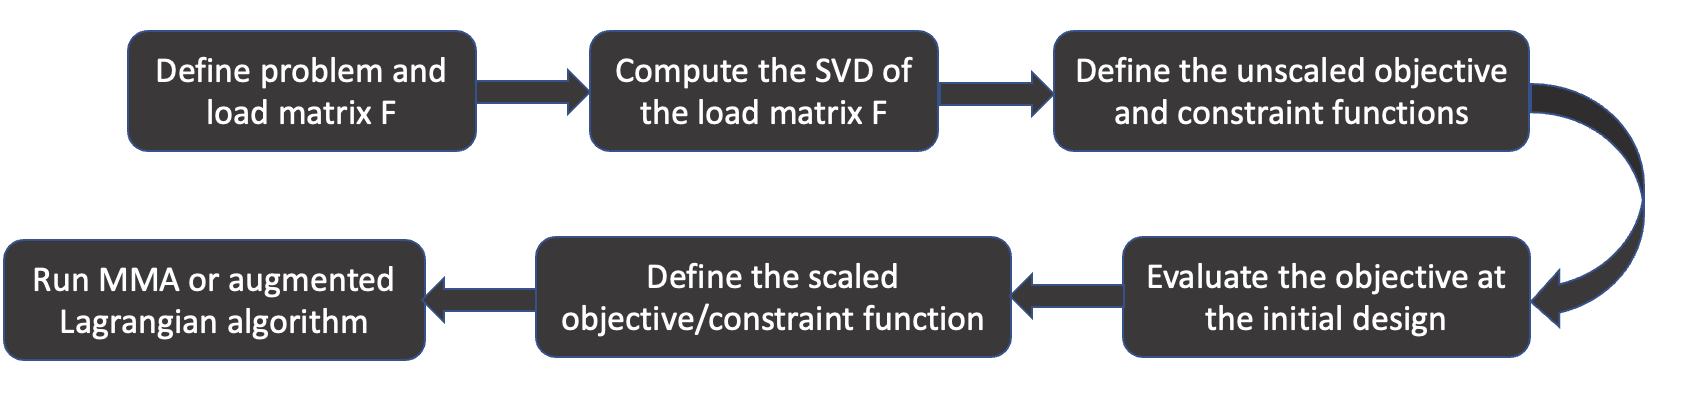
\includegraphics[width=\textwidth]{./images/robust_exact/flowchart.png}
      \caption{Flowchart of the experiments' workflow. Only the mean compliance objective, mean-std compliance objective or maximum compliance constraint are scaled by the inverse of their initial value. The volume function is not scaled.}
      \label{fig:flowchart}
    \end{figure}

    \subsubsection{Mean compliance minimization}

      To demonstrate the effectiveness of the proposed approaches, the 2D and 3D cantilever beam problems described in section \ref{sec:exp_impl} were solved using the proposed SVD-based methods. Table \ref{tab:mean_stats} shows the statistics of the final optimal solutions obtained by minimizing the mean compliance subject to the volume fraction constraint using the SVD-based method to evaluate the mean compliance. The optimal topologies are shown in Figures \ref{fig:mean} and \ref{fig:exact_mean_3d}.

      \begin{figure}
        \centering
        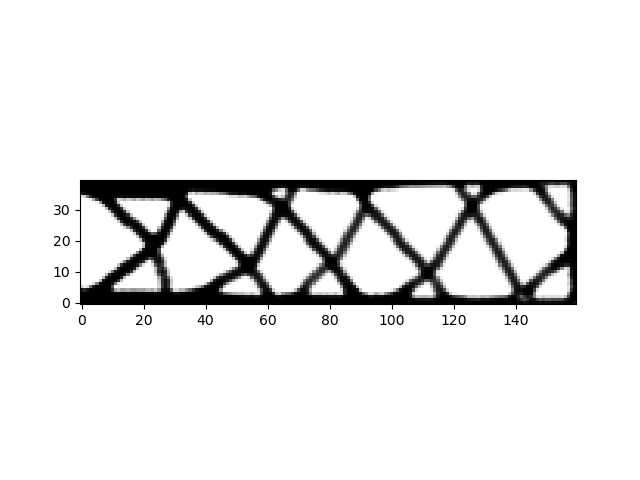
\includegraphics[width=\textwidth]{./images/robust_exact/exact_svd_mean_csimp.png}
        \caption{Optimal topology of the mean compliance minimization problem using continuation SIMP and the SVD-based method for evaluating the mean compliance.}
        \label{fig:mean}
      \end{figure}

      \begin{figure}
        \begin{subfigure}[t]{0.45\textwidth}
          \centering
          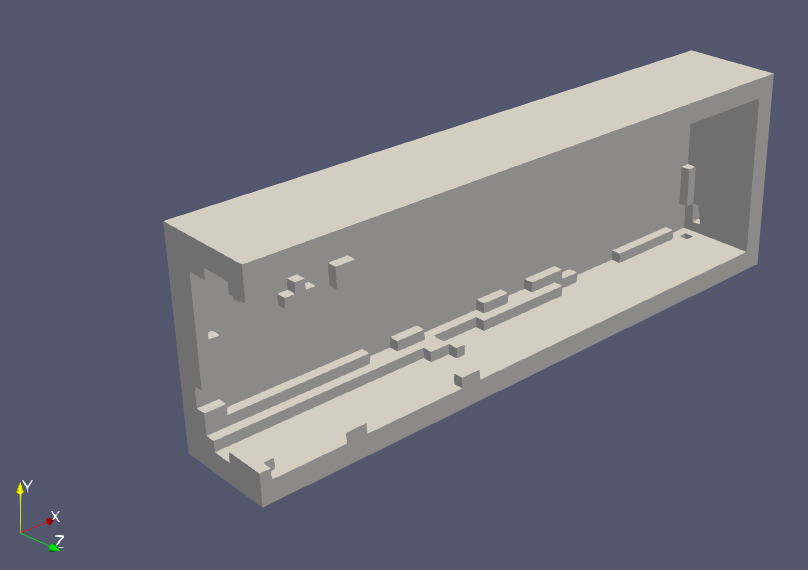
\includegraphics[width=1\textwidth]{./images/robust_exact/exact_mean_1.png}
          \caption{Left half}
        \end{subfigure}
        \begin{subfigure}[t]{0.45\textwidth}
          \centering
          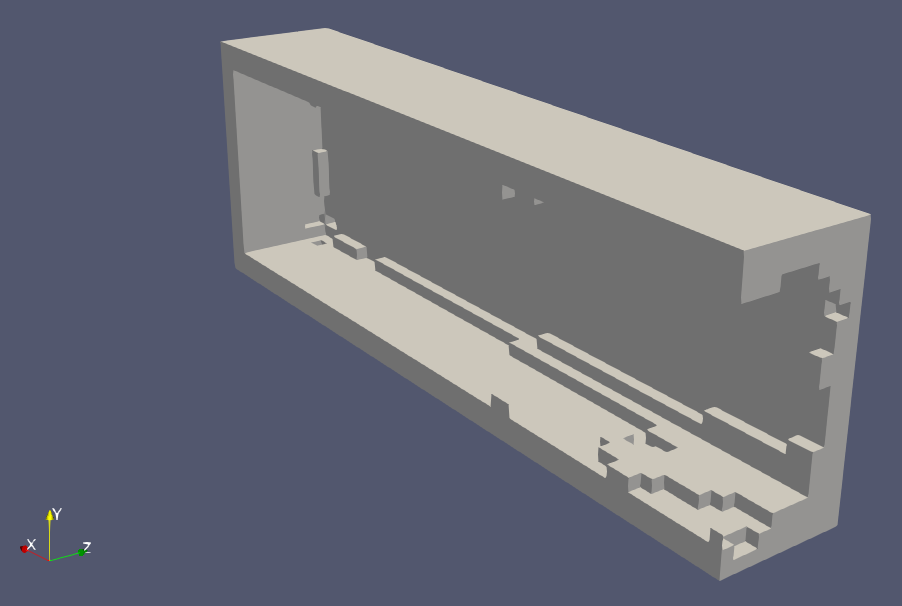
\includegraphics[width=1\textwidth]{./images/robust_exact/exact_mean_2.png}
          \caption{Right half}
        \end{subfigure}
        \caption{Cut views of the optimal topologies of the 3D mean compliance minimization problem using exact method with SVD.}
        \label{fig:exact_mean_3d}
      \end{figure}

      \begin{table}[h!]
       \centering
       \caption{Summary statistics of the load compliances of the optimal solutions of the 2D and 3D mean compliance minimization problems using the SVD-based method to evaluate the mean compliance.}
       \begin{tabular}{|c|c|c|}
        %1.1 - 0.7 - 0.5
        \hline
        Compliance Stat & 2D & 3D \\
        \hline
        \hline
        $\mu_C$ (Nmm) & 9392.8 & 22072.1 \\
        \hline
        $\sigma_C$ (Nmm) & 9688.8 & 16628.7 \\
        \hline
        $C_{max}$ (Nmm) & 125455.0 & 184055.0 \\
        \hline
        $C_{min}$ (Nmm) & 467.9 & 1785.8 \\
        \hline
        $V$ & 0.400 & 0.400 \\
        \hline
        $Time$ (s) & 491.5 & 3849.6 \\
        \hline
       \end{tabular}
       \label{tab:mean_stats}
      \end{table}

    \subsubsection{Mean-std compliance minimization}

      Similarly, Table \ref{tab:mean_std_stats} shows the statistics of the final solutions of the 2D and 3D mean-std minimization problems solved using the SVD-based method. The optimal topologies are shown in Figures \ref{fig:mean_std} and \ref{fig:exact_mean_std_3d}. The algorithm converged to reasonable, feasible designs. Additionally, as expected the mean-std minimization algorithm converged to solutions with lower compliance standard deviations but higher mean compliances compared to the mean minimization algorithm.

      \begin{figure}
        \centering
        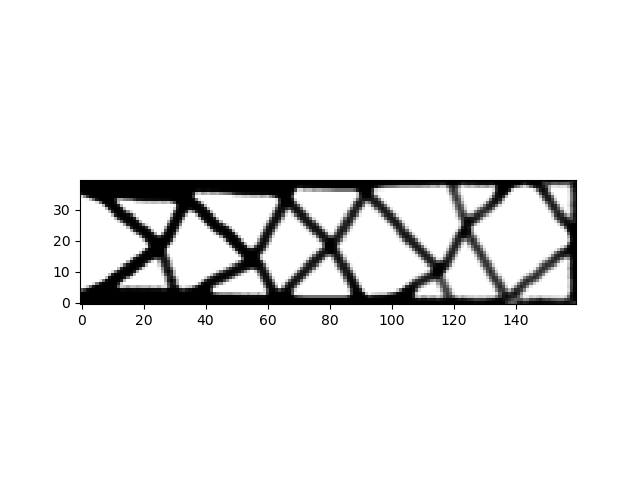
\includegraphics[width=\textwidth]{./images/robust_exact/exact_svd_mean_std_csimp.png}
        \caption{Optimal topology of the mean-std compliance minimization problem using continuation SIMP and the SVD-based method to compute the mean-std.}
        \label{fig:mean_std}
      \end{figure}

      \begin{figure}
        \begin{subfigure}[t]{0.45\textwidth}
          \centering
          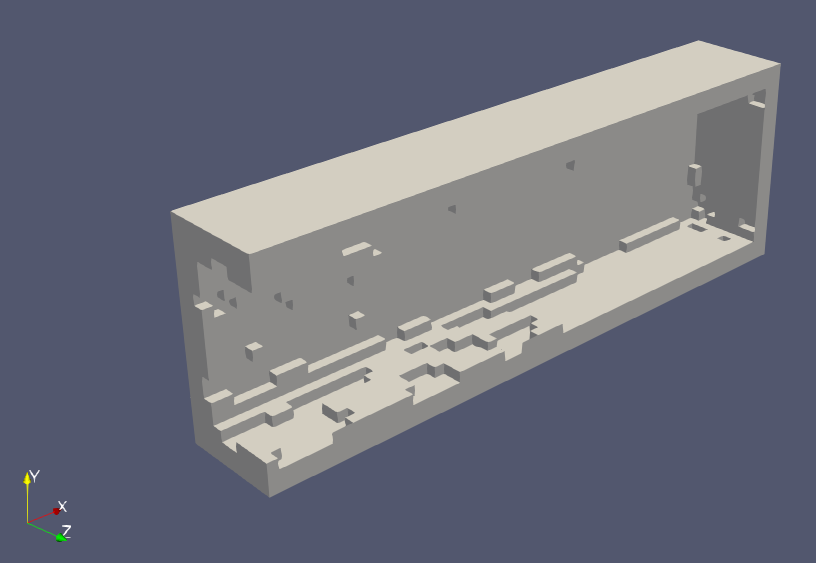
\includegraphics[width=1\textwidth]{./images/robust_exact/exact_mean_std_1.png}
          \caption{Left half}
        \end{subfigure}
        \begin{subfigure}[t]{0.45\textwidth}
          \centering
          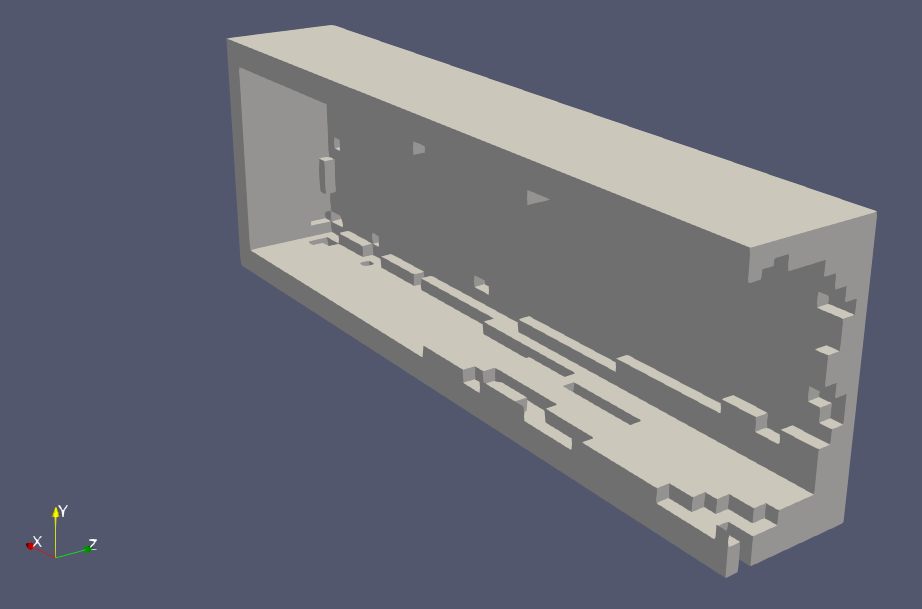
\includegraphics[width=1\textwidth]{./images/robust_exact/exact_mean_std_2.png}
          \caption{Right half}
        \end{subfigure}
        \caption{Cut views of the optimal topologies of the 3D mean-std compliance minimization problem using the exact method with SVD.}
        \label{fig:exact_mean_std_3d}
      \end{figure}

      \begin{table}[h!]
       \centering
       \caption{Summary statistics of the load compliances of the optimal solutions of the 2D and 3D mean-std compliance minimization problems using the SVD-based method to evaluate the mean-std compliance.}
       \begin{tabular}{|c|c|c|}
        \hline
        Compliance Stat & 2D & 3D \\
        \hline
        \hline
        $\mu_C (Nmm) $ & 9796.9 & 22216.7 \\
        \hline
        $\sigma_C (Nmm) $ & 9240.0 & 16220.2 \\
        \hline
        $\mu_C + 2.0 \sigma_C (Nmm) $ & 28283.7 & 54848.8 \\
        \hline
        $C_{max}$ (Nmm) & 117883.1 & 176153.2 \\
        \hline
        $C_{min}$ (Nmm) & 527.7 & 1872.0 \\
        \hline
        $V$ & 0.400 & 0.400 \\
        \hline
        Time (s) & 229.8 & 3528.2 \\
        \hline
       \end{tabular}
       \label{tab:mean_std_stats}
      \end{table}

      To highlight the effect of the multiple $m$ of the standard deviation in the objective $\mu_C + m \times \sigma_C$, the same problem was solved for different values of $m$. Figure \ref{fig:mean_std_profile} shows the profile of the mean and standard deviation of the compliance. Interestingly due to the non-convexity of the problem, increasing the standard deviation's multiple can sometimes lead to a simultaneous increase or reduction in the mean and standard deviation of the compliance. The different optimal topologies are shown in Figure \ref{fig:mean_m_std_2d}.

      \begin{figure}
        \centering
        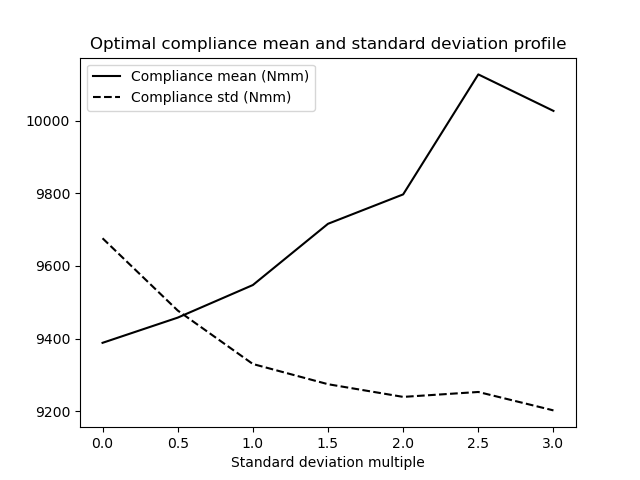
\includegraphics[width=\textwidth]{./images/robust_exact/mean_std_profile.png}
        \caption{Profile of the optimal mean and standard deviation of the compliance for different standard deviation multiples in the objective.}
        \label{fig:mean_std_profile}
      \end{figure}

      \begin{figure*}
        \begin{subfigure}[t]{0.45\textwidth}
          \centering
          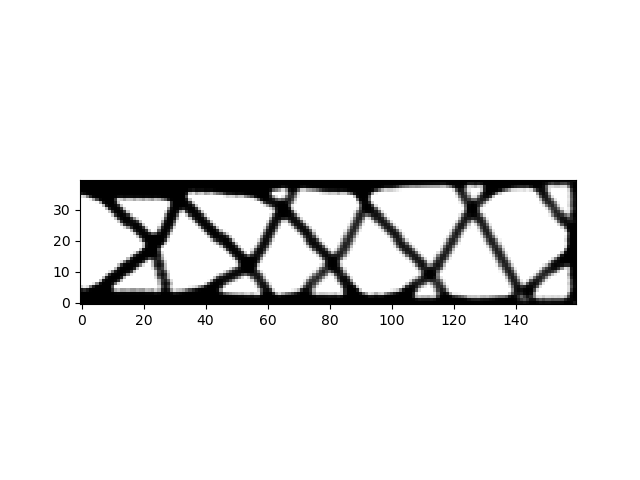
\includegraphics[width=1\textwidth]{./images/robust_exact/exact_svd_mean_0std_csimp.png}
          \caption{$m = 0$}
        \end{subfigure}
        \begin{subfigure}[t]{0.45\textwidth}
          \centering
          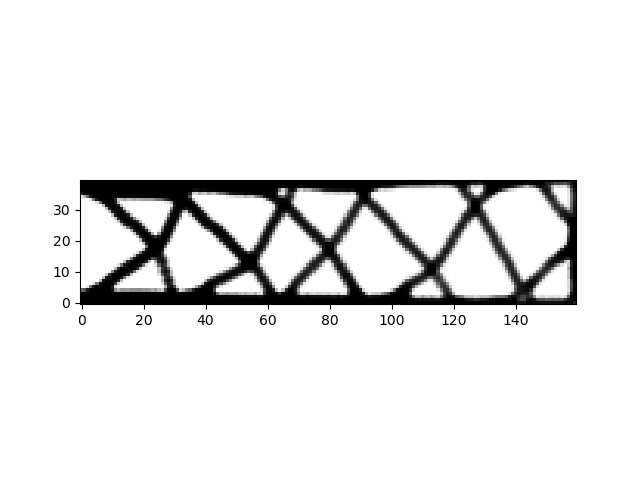
\includegraphics[width=1\textwidth]{./images/robust_exact/exact_svd_mean_5std_csimp.png}
          \caption{$m = 0.5$}
        \end{subfigure}
        \begin{subfigure}[t]{0.45\textwidth}
          \centering
          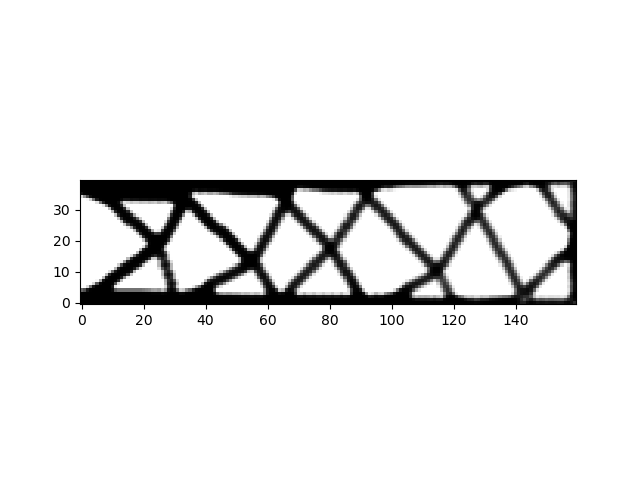
\includegraphics[width=1\textwidth]{./images/robust_exact/exact_svd_mean_10std_csimp.png}
          \caption{$m = 1.0$}
        \end{subfigure}
        \begin{subfigure}[t]{0.45\textwidth}
          \centering
          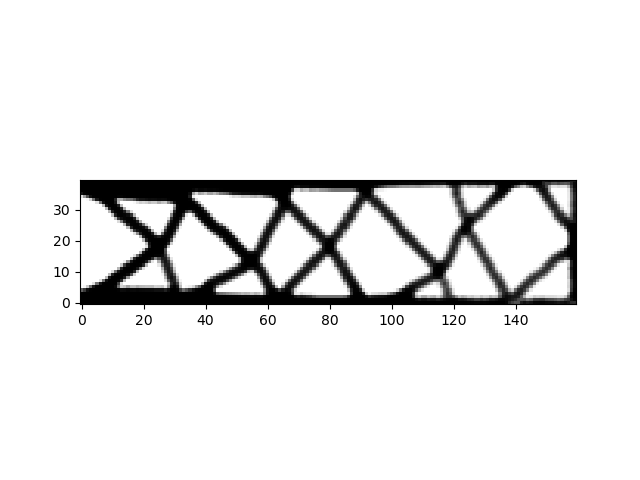
\includegraphics[width=1\textwidth]{./images/robust_exact/exact_svd_mean_15std_csimp.png}
          \caption{$m = 1.5$}
        \end{subfigure}
        \begin{subfigure}[t]{0.45\textwidth}
          \centering
          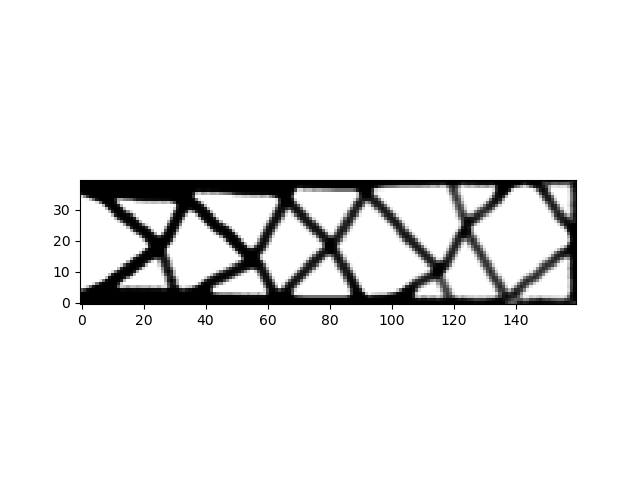
\includegraphics[width=1\textwidth]{./images/robust_exact/exact_svd_mean_20std_csimp.png}
          \caption{$m = 2.0$}
        \end{subfigure}
        \begin{subfigure}[t]{0.45\textwidth}
          \centering
          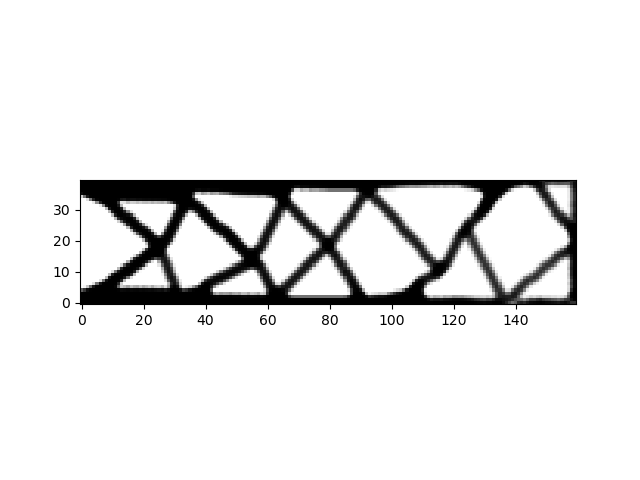
\includegraphics[width=1\textwidth]{./images/robust_exact/exact_svd_mean_25std_csimp.png}
          \caption{$m = 2.5$}
        \end{subfigure}
        \begin{subfigure}[t]{0.45\textwidth}
          \centering
          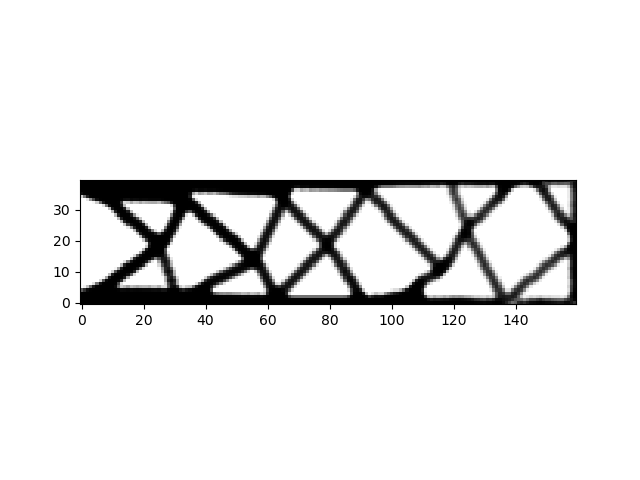
\includegraphics[width=1\textwidth]{./images/robust_exact/exact_svd_mean_30std_csimp.png}
          \caption{$m = 3.0$}
        \end{subfigure}
        \caption{Optimal topologies of the 2D mean-std compliance minimization problem using different standard deviation multiples $m$ in the objective $\mu_C + m \sigma_C$.}
        \label{fig:mean_m_std_2d}
      \end{figure*}

    \subsubsection{Maximum compliance constrained optimization}

      The 2D and 3D maximum compliance constrained volume minimization problems were solved using the SVD-based approach. The 2D optimal topology, shown in Figure \ref{fig:max}, had a volume fraction of 0.584 and a maximum compliance of 69847.0 Nmm and was reached in 662.7 s. The 3D optimal topology, shown in Figure \ref{fig:max_3d}, had a volume fraction of 0.791 and a maximum compliance of 68992.4 Nmm and was reached in 43740.6 s.

      \begin{figure}
        \centering
        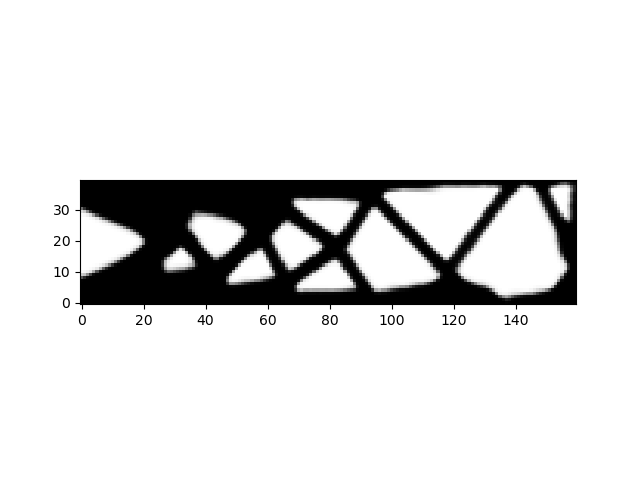
\includegraphics[width=\textwidth]{./images/robust_exact/exact_svd_max_csimp.png}
        \caption{Optimal topology of the volume minimization problem subject to a maximum compliance constraint using continuation SIMP and the augmented Lagrangian method with the exact SVD approach. The maximum compliance of the design above is 69847.0 Nmm and the volume fraction is 0.584.}
        \label{fig:max}
      \end{figure}

      \begin{figure}
        \centering
        \begin{subfigure}[t]{0.45\textwidth}
          \centering
          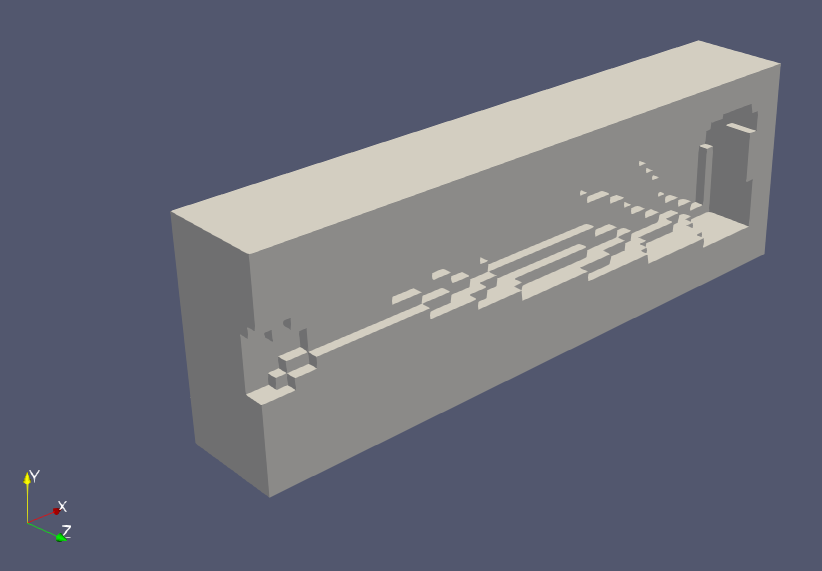
\includegraphics[width=1\textwidth]{./images/robust_exact/exact_max_1.png}
          \caption{Left half}
        \end{subfigure}
        \begin{subfigure}[t]{0.45\textwidth}
          \centering
          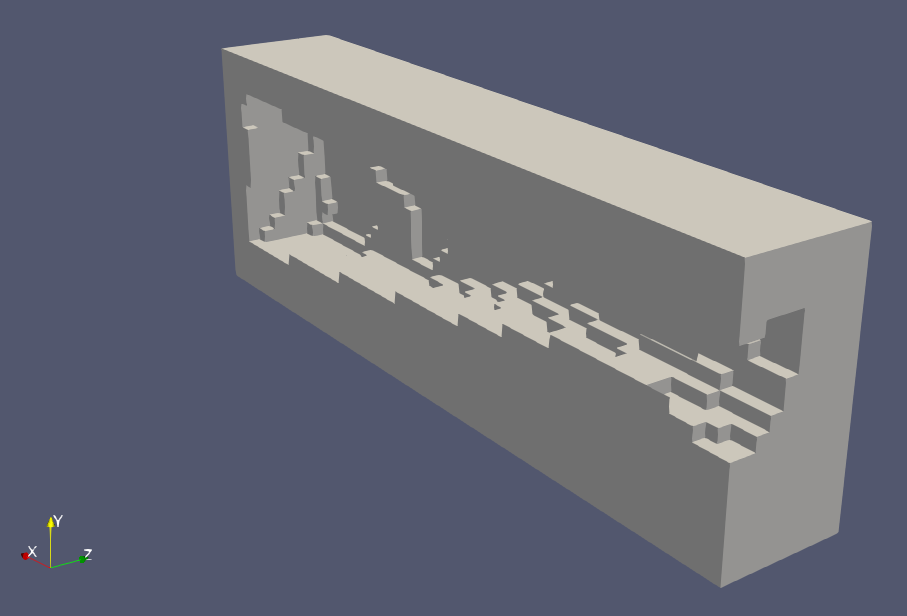
\includegraphics[width=1\textwidth]{./images/robust_exact/exact_max_2.png}
          \caption{Right half}
        \end{subfigure}
        \caption{Cut views of the 3D optimal topology of the volume minimization problem subject to a maximum compliance constraint using continuation SIMP and the augmented Lagrangian method with the exact SVD approach. The maximum compliance of the design above is 68992.4 Nmm and the volume fraction is 0.791.}
        \label{fig:max_3d}
      \end{figure}

\section{Conclusion} \label{sec:conclusion}

  In this chapter, a number of exact methods were proposed to handle load uncertainty in compliance topology optimization problems where the uncertainty is described in the form of a set of finitely many loading scenarios. By exploiting low rank structures in loading scenarios, significant performance improvements were achieved using novel SVD-based methods. Such improvement was demonstrated via complexity analysis and computational experiments. The methods presented here are fundamentally data-driven in the sense that no probability distributions or domains are assumed for the loading scenarios. This sets this work apart from most of the literature in the domain of stochastic and robust topology optimization where a distribution or domain is assumed. Additionally, the methods proposed here were shown to be particularly suitable with the augmented Lagrangian algorithm when dealing with maximum compliance constraints.

\newpage
